\begin{frame}\frametitle{Chamfer matching}
    \begin{itemize}
        \item Задача: научиться по контуру предмета находить этот предмет на изображении.
        \pause
        \item Рассмотренный подход к решению описан в статье
        Ming-Yu Liu, Oncel Tuzel, Ashok Veeraraghavan, Rama Chellappa. Fast Directional Chamfer Matching
    \end{itemize}
\end{frame}

\begin{frame}\frametitle{Алгоритм}
    \begin{itemize}
        \item С помощью алгоритма Кэнни найти на изображении границы между объектами.
        \pause
        \item Представить границы на изображении и контур предмета в виде набора отрезков.
        Такое представление удобно для дальнейших оптимизаций.
        \pause
        \item Для каждого возможного наложения контура на изображение посчитать эвристическую функцию отклонения.
        \pause
        \item Среди всех наложений выбрать одно с минимальным значением функции.
    \end{itemize}
\end{frame}

\begin{frame}\frametitle{Алгоритм Кэнни}
    \begin{itemize}
        \item Алгоритм Кэнни получает на вход изображение, как функцию интенсивности от двух переменных.
        \pause
        \item Для каждого пикселя вычисляется приближенное значение градиента этой функции в данном пикселе.
        \pause
        \item Пиксели с высоким значением модуля градиента объявляются граничными.
        \pause
        \item В работе был использован готовый алгоритм из библиотеки OpenCV.
    \end{itemize}
\end{frame}


\begin{frame}\frametitle{Неустойчивость к помехам}
    \begin{center}
        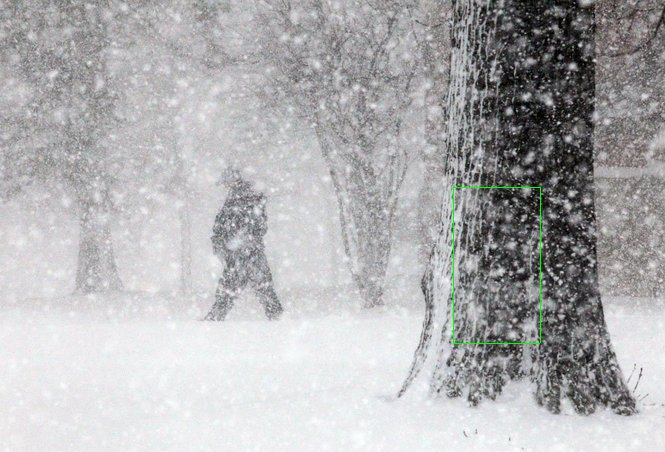
\includegraphics[height=6cm]{veselov_imgs/occurrence2.jpg}
    \end{center}
\end{frame}

\begin{frame}\frametitle{Заключение о Chamfer matching}
    Во время работы над проектом:
    \begin{itemize}
        \item Были изучены статьи на тему
        <<компьютерного зрения>> (Chamfer matching, Canny algorithm), а также
        вероятностного поиска некоторой модели среди помех (RANSAC).
        
        \item Была написана реализация Chamfer matching на языке Python с
        использованием пакетов numpy и cv2.
        
        \item Для хранения исходного кода использовался GitHub.
    \end{itemize}
\end{frame}

Задача
Алгоритм
-Определение ключевых точек
-Сопоставление ключевых точек
-PnP
-склонен к ошибкам, поэтому RANSAC (Random sample consensus)
Определение ключевых точек
-Точки, которые обладают некоторыми важными свойствами
-Устойчивость к деформациям, точность локализации
Сопоставление ключевых точек
-Вычисление дескрипторов (вектор 128)
-Сопоставление точек расстояние между дескрипторами которых минимально
RANSAC

